\section{Array Architecture}
As was mentioned in the previous section, points with the same TDOA to two fixed locations form a hyperbola on a 2D plane. However, in practical systems we can only measure TDOA up to a precision. Therefore we look at all points with difference of distance close to some target value within measurement error $\epsilon$. This $\epsilon$ represents accuracy on the measurement of difference of distances, and in practice it is related to sampling rate and estimation techniques. In this section we evaluate the impact of difference of distance estimation on localization accuracy.

\begin{figure}[]
  \centering
  \begin{subfigure}[]{.23\textwidth}
    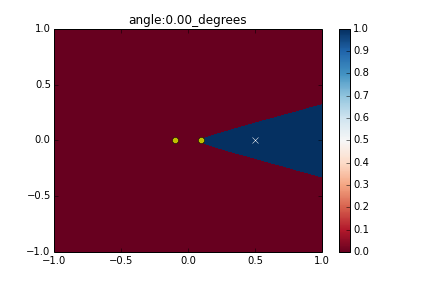
\includegraphics[width=\textwidth]{sim/sim_2_1}
    \caption{source at $(r=50$ cm,$\theta = 0$ degrees$)$}
  \end{subfigure}
  \begin{subfigure}[]{.23\textwidth}
    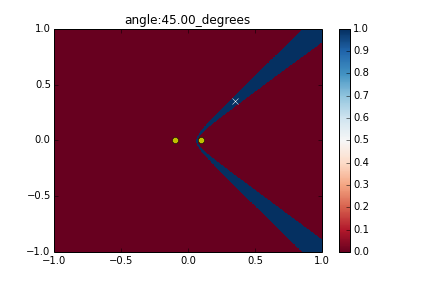
\includegraphics[width=\textwidth]{sim/sim_2_2}
    \caption{source at $(r=50$ cm,$\theta = 45$ degrees$)$}
  \end{subfigure}
  \begin{subfigure}[]{.23\textwidth}
    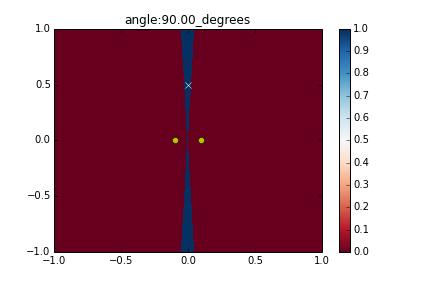
\includegraphics[width=\textwidth]{sim/sim_2_3}
    \caption{source at $(r=50$ cm,$\theta = 90$ degrees$)$}
  \end{subfigure}
  \caption{Uncertainty region}
  \label{fig:sim_2_5}
\end{figure}

To see how precision affects localization accuracy, we simulated two microphones placed at: $M_1:(x=-10\mbox{ cm},y=0\mbox{ cm})$ and $M_2:(x=10\mbox{ cm},y=0\mbox{ cm})$. A test sound source is emitted at point $P$ which is $50$ centimeters away from the origin $(0,0)$. Let $2a$ denote the difference of distance between $P$ and two microphones:
\[
2a = P M_1 - P M_2 
\]
, then fig~\ref{fig:sim_2_5} shows the region $R$ where all points have difference of distance to two microphones close to $a$ within $1$ cm:
\[
R=\{\hat P: |(\hat P M_1 - \hat P M_2) - 2a|< 1 \mbox{ cm}\}
\]
Intuitively, points in $R$ have difference of distance to two microphones very similar to each other. Looking at fig~\ref{fig:sim_2_5}, we can still see that $R$ has the shape of a hyperbola, but with an uncertainty region around it. The thickness of the uncertainty region is not uniform around the hyperbola, the farther away the point is, the larger the uncertainty region becomes. This indicates for the same delta distance movement it will generate smaller difference of distance change when the source is farther away from the array. The size of the uncertainty region is also angle dependent: points closer to the line connecting microphones have larger region compared to points close to the line bisecting microphones. 

This can also be seen analytically. Assuming two microphones are placed on the x-axis at $M_1:(-c,0)$ and $M2:(c,0)$. All points $P:(x,y)$ with difference of distance $ |PM_1 - PM_2| = 2a$ satisfies:
\begin{eqnarray}\label{eqn:hyperbola}
\frac{x^2}{a^2} - \frac{y^2}{c^2-a^2} = 1
\end{eqnarray}
To see how difference of distance changes with respect to distance, we can expand the equation and find partial differential $\frac{\partial a}{\partial x}$:
\begin{eqnarray}\label{eqn:derivative}
\frac{\partial a}{\partial x} = \frac{x(c^2-a^2)}{a(x^2+y^2+c^2)-2a^3}
\end{eqnarray}
Since all points in equation~\ref{eqn:derivative} must lie on the hyperbola, we can substitute~\ref{eqn:hyperbola} into~\ref{eqn:derivative}:
\begin{eqnarray}\label{eqn:derivativeF}
\frac{\partial a}{\partial x} = \frac{c^2-a^2}{\frac{c^2}{a}x - \frac{a^3}{x}}
\end{eqnarray}

The denominator of equation~\ref{eqn:derivativeF} increases monotonically as $|x|$ increases, which indicates $\frac{\partial a}{\partial x}$ decreases as we move farther away along the hyperbola. The same distance move $\delta x$ would generate smaller change in difference of distance $a$ when the source is farther away from the microphones. 

\begin{figure*}[]
  \centering
  \begin{subfigure}[]{.3\textwidth}
    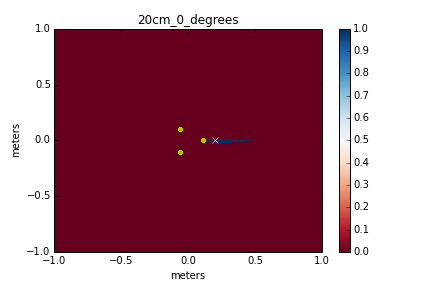
\includegraphics[width=\textwidth]{sim/result_20cm_0_degrees}
    \caption{0 degrees}
  \end{subfigure}
  \begin{subfigure}[]{.3\textwidth}
    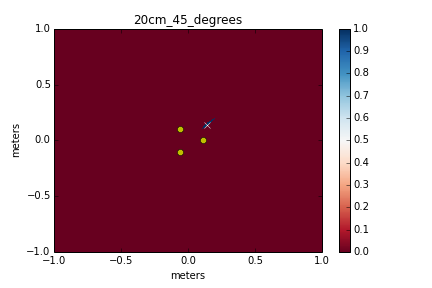
\includegraphics[width=\textwidth]{sim/result_20cm_45_degrees}
    \caption{45 degrees}
  \end{subfigure}
  \begin{subfigure}[]{.3\textwidth}
    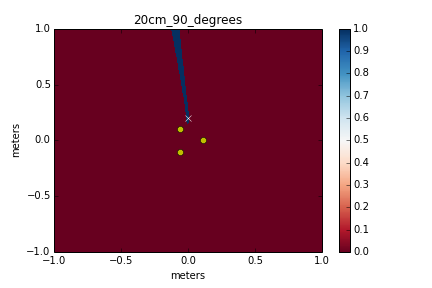
\includegraphics[width=\textwidth]{sim/result_20cm_90_degrees}
    \caption{90 degrees}
  \end{subfigure}
  \begin{subfigure}[]{.3\textwidth}
    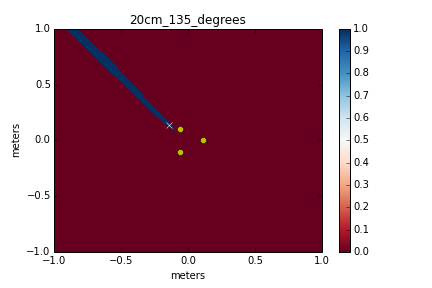
\includegraphics[width=\textwidth]{sim/result_20cm_135_degrees}
    \caption{135 degrees}
  \end{subfigure}
  \begin{subfigure}[]{.3\textwidth}
    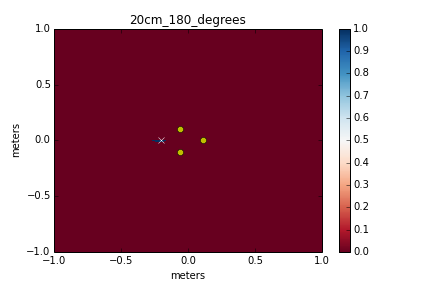
\includegraphics[width=\textwidth]{sim/result_20cm_180_degrees}
    \caption{180 degrees}
  \end{subfigure}
  \caption{$20$cm equilateral triangle array. Source is $20$cm away from the array}
  \label{fig:sim_3_2}
\end{figure*}

\begin{figure*}[]
  \centering
  \begin{subfigure}[]{.3\textwidth}
    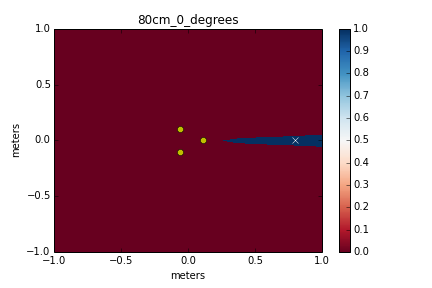
\includegraphics[width=\textwidth]{sim/result_80cm_0_degrees}
    \caption{0 degrees}
  \end{subfigure}
  \begin{subfigure}[]{.3\textwidth}
    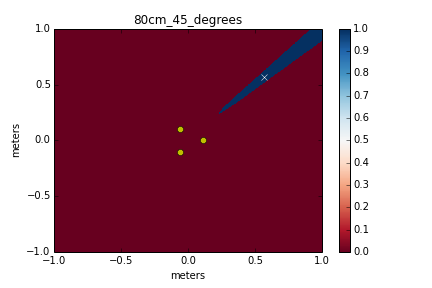
\includegraphics[width=\textwidth]{sim/result_80cm_45_degrees}
    \caption{45 degrees}
  \end{subfigure}
  \begin{subfigure}[]{.3\textwidth}
    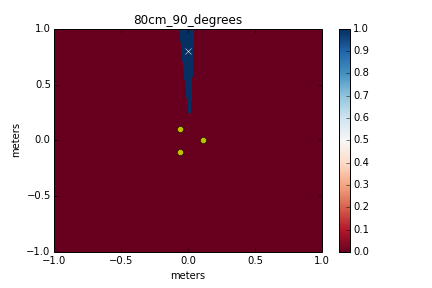
\includegraphics[width=\textwidth]{sim/result_80cm_90_degrees}
    \caption{90 degrees}
  \end{subfigure}
  \begin{subfigure}[]{.3\textwidth}
    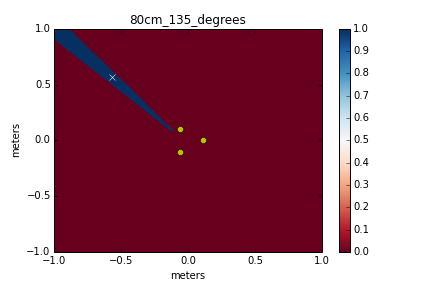
\includegraphics[width=\textwidth]{sim/result_80cm_135_degrees}
    \caption{135 degrees}
  \end{subfigure}
  \begin{subfigure}[]{.3\textwidth}
    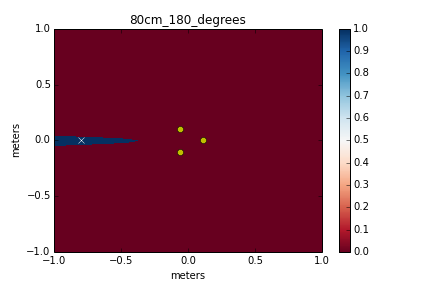
\includegraphics[width=\textwidth]{sim/result_80cm_180_degrees}
    \caption{180 degrees}
  \end{subfigure}
  \caption{$20$ cm equilateral triangle array. Source is $80$ cm away from the array}
  \label{fig:sim_3_8}
\end{figure*}

With more than two microphones, each pair of microphones generates a hyperbolic region and localization becomes finding the intersection of hyperbolic regions. The smaller the intersection region, the better the localization accuracy. To see how accuracy changes with array placement and sound source location, three microphones are placed at the three vertices of an $20$ cm equilateral triangle. An audio source is placed at $20$ cm away from the center of the array. Fig~\ref{fig:sim_3_2} shows the intersection of regions for $5$ different placement of the sound source. It can be seen that accuracy decreases when sound source becomes close to the line connecting any two microphones. This observation is consistent with the two microphone case, since points close to lines connecting microphones have a larger uncertainty region.

To see how sound source distance affects localization accuracy, the same simulation is carried out with the sound source moved from $20$ cm to $80$ cm away from the center of the array. Results are presented in fig~\ref{fig:sim_3_8}. Comparing with fig~\ref{fig:sim_3_2}, accuracy decreases as the distance to the array increases. This is also consistent with our observation in $2$ microphone case where sources farther away would result in larger uncertainty region.

\begin{figure*}[]
  \centering
  \begin{subfigure}[]{.3\textwidth}
    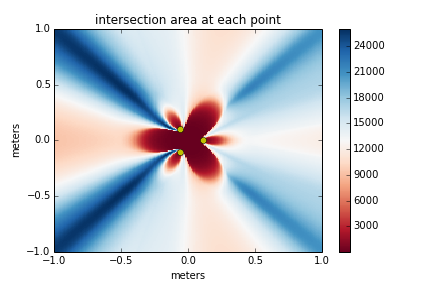
\includegraphics[width=\textwidth]{sim/result_intersection_area_at_each_point_3_center}
    \caption{$3$ microphones placed at vertices of an $20$cm equilateral triangle. Average error is $18.6$ cm}
    \label{fig:sim_hm_3}
  \end{subfigure}
  \begin{subfigure}[]{.3\textwidth}
    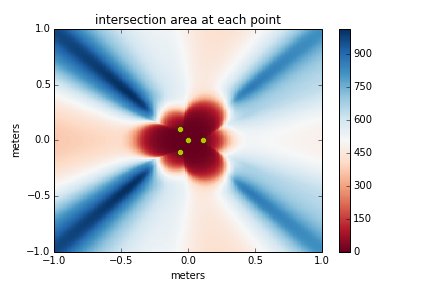
\includegraphics[width=\textwidth]{sim/result_intersection_area_at_each_point_3_p1}
    \caption{another microphone added at origin. Average error is $17.1$ cm}
    \label{fig:sim_hm_3_p1}
  \end{subfigure}
  \begin{subfigure}[]{.3\textwidth}
    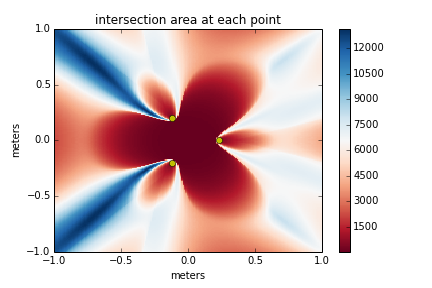
\includegraphics[width=\textwidth]{sim/result_intersection_area_at_each_point_3_2x}
    \caption{$3$ microphones placed at vertices of an $40$cm equilateral triangle. Average error is $10.04$ cm}
    \label{fig:sim_hm_3_2x}
  \end{subfigure}
  \begin{subfigure}[]{.3\textwidth}
    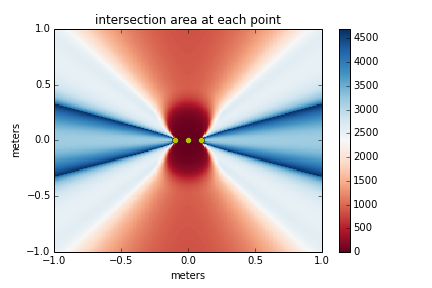
\includegraphics[width=\textwidth]{sim/result_intersection_area_at_each_point_3_line}
    \caption{$3$ microphones placed in a line. Total length is $20$ cm. Average error is $55.05$ cm}
    \label{fig:sim_hm_3_line}
  \end{subfigure}
  \begin{subfigure}[]{.3\textwidth}
    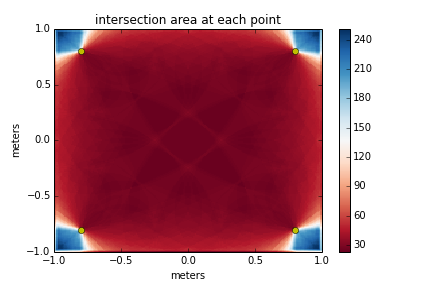
\includegraphics[width=\textwidth]{sim/result_intersection_area_at_each_point_4corner}
    \caption{$4$ microphones placed at $4$ corners of the region. Average error is $0.05$ cm}
    \label{fig:sim_hm_4}
  \end{subfigure}
  \begin{subfigure}[]{.3\textwidth}
    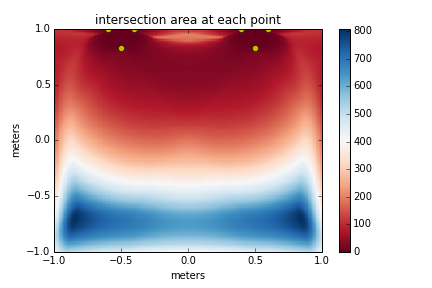
\includegraphics[width=\textwidth]{sim/result_intersection_area_at_each_point_2a}
    \caption{two $3$ microphone arrays placed $1$ meter apart. Average error is $2.60$ cm}
    \label{fig:sim_hm_2_array}
  \end{subfigure}
  \caption{Accuracy for different array configurations}
  \label{fig:sim_hm}
\end{figure*}

Each microphone pair generates a hyperbolic region, and the intersection area of these regions is a measure of the localization accuracy. To evaluate an array's accuracy in a region, we can place sound source at predetermined grid points in the region and look at the intersection area for each tested point in the grid. The center location of intersection region can be used as the localization estimate to calculate localization error. Results for a few different microphone array configurations are presented in fig~\ref{fig:sim_hm}.

Fig~\ref{fig:sim_hm_3} shows the accuracy when microphones are placed at the three vertices of a $20$ cm equilateral triangle. The region inside the array has good accuracy. However, for regions along the line connecting any two microphones, the accuracy drops significantly. Average error across the region is $18.6$ cm.

To evaluate how adding one microphone(without increasing the array size) improves accuracy, another microphone is added to the array at $(0,0)$. Result is presented in fig~\ref{fig:sim_hm_3_p1}. Addition of the new microphone only slightly improved the accuracy around the array region. Average error dropped from $18.6$ cm to $17.1$ cm. Regions near lines connecting microphones still have significantly larger uncertainty region.

To evaluate the array size's impact on accuracy, the size of the original array (as in fig~\ref{fig:sim_hm_3}) is increased by a factor of $2$. The result is presented in fig~\ref{fig:sim_hm_3_2x}. The overall uncertainty area decreased across the region. Average error improved to $10.04$ cm. 

In fig~\ref{fig:sim_hm_3_line}, three microphones are placed $10$ cm apart from each other on the x-axis. Error heatmap shows high uncertainty on the x axis, and the overall accuracy is not as good as that with three microphones placed in a triangle. The average error is $55.05$ cm. 

To further increase the distance between microphones, we placed four microphones at four corners of the region. Fig~\ref{fig:sim_hm_4} shows the result. With this configuration, accuracy is consistently good across the region. The average error is $0.05$ cm.  However, placing microphones far apart at corners of the region requires accurate placement of all four individual microphones. The system is less portable compared to small arrays with microphones near each other. Placing microphones far apart from each other also causes problems in TDOA estimation, because sampling of microphones in the same array requires synchronized clock.

To avoid the need to accurately place microphones at far distances(as required by fig~\ref{fig:sim_hm_4}), we explored configuration with two arrays. Two $3$ microphone array are placed $1$ meter apart and the result is presented in fig~\ref{fig:sim_hm_2_array}.  The result indicates that this configuration has good accuracy when source is close to the arrays. Accuracy decreases as sound source moves outside of the one meter by one meter region. The average error is $2.60$ cm. 

With the simulation results, we decided to build the two array system as described in fig~\ref{fig:sim_hm_2_array}. The setup is reasonably portable (compared to fig~\ref{fig:sim_hm_4}), while at the same time having significantly better accuracy compared to one array systems.
